%%%%%%%%%%%%%%%%%%%%%%%%%%%%%%%%%%%%%%%%%
% Programming/Coding Assignment
% LaTeX Template
%
% This template has been downloaded from:
% http://www.latextemplates.com
%
% Original author:
% Ted Pavlic (http://www.tedpavlic.com)
%
% This template uses a Perl script as an example snippet of code, most other
% languages are also usable. Configure them in the "CODE INCLUSION 
% CONFIGURATION" section.
%
%%%%%%%%%%%%%%%%%%%%%%%%%%%%%%%%%%%%%%%%%

%----------------------------------------------------------------------------------------
%	PACKAGES AND OTHER DOCUMENT CONFIGURATIONS
%----------------------------------------------------------------------------------------

\documentclass{article}
%\documentclass[english,a4paper,twoside]{amsart}

\usepackage{fancyhdr} % Required for custom headers
\usepackage{lastpage} % Required to determine the last page for the footer
\usepackage{extramarks} % Required for headers and footers
\usepackage[usenames,dvipsnames]{color} % Required for custom colors
\usepackage{graphicx} % Required to insert images
\usepackage{listings} % Required for insertion of code
\usepackage{courier} % Required for the courier font
\usepackage{gensymb} % degree symbol

\usepackage[utf8]{inputenc}
\usepackage[T1]{fontenc}

\usepackage{amsmath}
\newcommand*{\maxeq}{\stackrel{\text{min}}{=}}
\newcommand*{\mineq}{\stackrel{\text{max}}{=}}

% Margins
\topmargin=-0.45in
\evensidemargin=0in
\oddsidemargin=0in
\textwidth=6.5in
\textheight=9.0in
\headsep=0.25in

\linespread{1.1} % Line spacing

% Set up the header and footer
\pagestyle{fancy}
\lhead{\hmwkAuthorName} % Top left header
\chead{\hmwkClass : \hmwkTitle} % Top center head
\rhead{\firstxmark} % Top right header
\lfoot{\lastxmark} % Bottom left footer
\cfoot{} % Bottom center footer
\rfoot{Page\ \thepage\ of\ \protect\pageref{LastPage}} % Bottom right footer
\renewcommand\headrulewidth{0.4pt} % Size of the header rule
\renewcommand\footrulewidth{0.4pt} % Size of the footer rule

\setlength\parindent{0pt} % Removes all indentation from paragraphs

%----------------------------------------------------------------------------------------
%	CODE INCLUSION CONFIGURATION
%----------------------------------------------------------------------------------------

\definecolor{MyDarkGreen}{rgb}{0.0,0.4,0.0} % This is the color used for comments
\lstloadlanguages{Perl} % Load Perl syntax for listings, for a list of other languages supported see: ftp://ftp.tex.ac.uk/tex-archive/macros/latex/contrib/listings/listings.pdf
\lstset{%language=Perl, % Use Perl in this example
        frame=single, % Single frame around code
        basicstyle=\small\ttfamily, % Use small true type font
        keywordstyle=[1]\color{Blue}\bf, % Perl functions bold and blue
        keywordstyle=[2]\color{Purple}, % Perl function arguments purple
        keywordstyle=[3]\color{Blue}\underbar, % Custom functions underlined and blue
        identifierstyle=, % Nothing special about identifiers                                         
        commentstyle=\usefont{T1}{pcr}{m}{sl}\color{MyDarkGreen}\small, % Comments small dark green courier font
        stringstyle=\color{Purple}, % Strings are purple
        showstringspaces=false, % Don't put marks in string spaces
        tabsize=5, % 5 spaces per tab
        %
        % Put standard Perl functions not included in the default language here
        morekeywords={rand},
        %
        % Put Perl function parameters here
        morekeywords=[2]{on, off, interp},
        %
        % Put user defined functions here
        morekeywords=[3]{test},
       	%
        morecomment=[l][\color{Blue}]{...}, % Line continuation (...) like blue comment
        numbers=left, % Line numbers on left
        firstnumber=1, % Line numbers start with line 1
        numberstyle=\tiny\color{Blue}, % Line numbers are blue and small
        stepnumber=5 % Line numbers go in steps of 5
}

% Creates a new command to include a perl script, the first parameter is the filename of the script (without .pl), the second parameter is the caption
\definecolor{background}{rgb}{0.98, 1, 1}
\newcommand{\shellcmd}[1]{
	\texttt{\# cwb-nc> #1}\\
}
\newcommand{\perlscript}[2]{
\begin{itemize}
	\item[]\lstinputlisting[backgroundcolor=\color{background},stepnumber=1,caption=#2,label=#1]{#1}
\end{itemize}
}

%----------------------------------------------------------------------------------------
%	DOCUMENT STRUCTURE COMMANDS
%	Skip this unless you know what you're doing
%----------------------------------------------------------------------------------------

% Header and footer for when a page split occurs within a problem environment
\newcommand{\enterProblemHeader}[1]{
\nobreak\extramarks{#1}{#1 continued on next page\ldots}\nobreak
\nobreak\extramarks{#1 (continued)}{#1 continued on next page\ldots}\nobreak
}

% Header and footer for when a page split occurs between problem environments
\newcommand{\exitProblemHeader}[1]{
\nobreak\extramarks{#1 (continued)}{#1 continued on next page\ldots}\nobreak
\nobreak\extramarks{#1}{}\nobreak
}

\setcounter{secnumdepth}{0} % Removes default section numbers
\newcounter{homeworkProblemCounter} % Creates a counter to keep track of the number of problems

\newcommand{\homeworkProblemName}{}
\newenvironment{homeworkProblem}[1][Problem \arabic{homeworkProblemCounter}]{ % Makes a new environment called homeworkProblem which takes 1 argument (custom name) but the default is "Problem #"
\stepcounter{homeworkProblemCounter} % Increase counter for number of problems
\renewcommand{\homeworkProblemName}{#1} % Assign \homeworkProblemName the name of the problem
\section{\homeworkProblemName} % Make a section in the document with the custom problem count
\enterProblemHeader{\homeworkProblemName} % Header and footer within the environment
}{
\exitProblemHeader{\homeworkProblemName} % Header and footer after the environment
}

\newcommand{\problemAnswer}[1]{ % Defines the problem answer command with the content as the only argument
\noindent\framebox[\columnwidth][c]{\begin{minipage}{0.98\columnwidth}#1\end{minipage}} % Makes the box around the problem answer and puts the content inside
}

\newcommand{\homeworkSectionName}{}
\newenvironment{homeworkSection}[1]{ % New environment for sections within homework problems, takes 1 argument - the name of the section
\renewcommand{\homeworkSectionName}{#1} % Assign \homeworkSectionName to the name of the section from the environment argument
\subsection{\homeworkSectionName} % Make a subsection with the custom name of the subsection
\enterProblemHeader{\homeworkProblemName\ [\homeworkSectionName]} % Header and footer within the environment
}{
\enterProblemHeader{\homeworkProblemName} % Header and footer after the environment
}

%----------------------------------------------------------------------------------------
%	NAME AND CLASS SECTION
%----------------------------------------------------------------------------------------

\newcommand{\hmwkTitle}{Project\ \#2} % Assignment title
\newcommand{\hmwkClass}{Modeling and Verification} % Course/class
\newcommand{\hmwkClassInstructor}{Anna Ingolfsdóttir} % Teacher/lecturer
\newcommand{\hmwkAuthorName}{Þröstur and Sævar} % Your name

%----------------------------------------------------------------------------------------
%	TITLE PAGE
%----------------------------------------------------------------------------------------

\title{
\vspace{2in}
\textmd{\textbf{\hmwkClass:\ \hmwkTitle}}\\
\vspace{0.1in}\large{\textit{\hmwkClassInstructor}}
\vspace{3in}
}

\author{\textbf{\hmwkAuthorName}}
\date{} % Insert date here if you want it to appear below your name

%----------------------------------------------------------------------------------------

\begin{document}

\maketitle

%----------------------------------------------------------------------------------------
%	TABLE OF CONTENTS
%----------------------------------------------------------------------------------------

%\setcounter{tocdepth}{1} % Uncomment this line if you don't want subsections listed in the ToC

\newpage

%----------------------------------------------------------------------------------------
%	PROBLEM 1
%----------------------------------------------------------------------------------------

% To have just one problem per page, simply put a \clearpage after each problem

\section{The Problem}
    A simple vacuum cleaner robot moves around a $3\times3$ room. The robot can only turn right or move forward and can only decide which action to take based on it's current location and direction. The robot starts in position $(0,0)$ facing north and must be able to move around the room such that it visits every cell infinitely often if allowed to run indefinitely. The robot follows a set of rules (called configurations in this report) where each individual rule states if the robot is in a specific cell, facing a specific direction, then it should move forward or turn. In this report, we use the modeling tool, \textit{Uppaal}, to find the configurations that solve this problem.

\section{The Model}
    We want to create a model that can examine all possible configurations, subject to some constraints, and give a configuration that solves the problem, or verify that no such configuration exists. There are 9 cells in the room and for each cell we have 4 directions which gives a total of 36 different states. Each state can have one of three rules (turn, move or undefined) and so we have a total of $3^{36}$ distinct configurations that can be defined for the vacuum robot and it is therefore not feasible to check each configuration individually. In order to decrease the size of the search space of the model, we delay the definition of individual rules for as long as possible and only define them right before they are used. This means we will not define rules for states that are unreachable and when we reject a configuration, we also reject all configuration that contain the rules of the rejected one. This drastically reduces the search space and the model can answer queries instantly.

    Figure \ref{fig:model} shows the uppaal automaton that defines the behaviour of the model. It begins by initializing the internal variables and setting any constraints that we define (hard coded rules) and then moves into the main location. If a rule is defined for the current state, it follows this rule, otherwise it non-deterministically chooses a rule for the current state. Before the model moves forward or turns, it must wait for 1 or 5 time units, respectivly, but this models the time it takes to perform these actions.

    \begin{figure}[h!]
        \caption{The Uppaal Model}
        \centering
        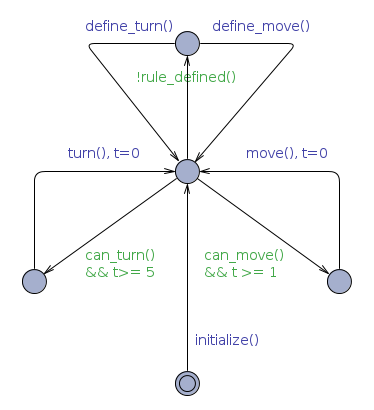
\includegraphics[width=0.5\textwidth]{model.png}
        \label{fig:model}
    \end{figure}

    The current state is stored in three internal variables, \texttt{x,y} and \texttt{dir} for the direction. We also store a single rule for each state where a rule can be either \texttt{TURN}, \texttt{MOVE} or \texttt{UNDEF}. The model also contains a number of internal functions that it uses during it's execution.
    
    The \texttt{initialize} function sets the current state to the starting state (position $(0,0)$ and facing north) and sets every rule to \texttt{UNDEF}. If we want to add constraints to the rules (e.g. fix the  Wooldridge rules) we define them in the initialize function by hardcoding rules for specific states. The function also marks every cell as not being visited so that we can verify that a configuration sends the vacuum robot to every cell in the room.

    \texttt{can\_move} and \texttt{can\_turn} return true if the corresponding rule is defined for the current state  and the new state will be not be inconsistent.

    \texttt{turn} simply updates the direction of the vacuum but \texttt{move} moves the vacuum forward in the direction it is facing and markes the new cell as visited. Since the vacuum begins in cell $(0,0)$, it will not be marked as visited unless the vacuum cleaner leaves this cell and later reenters it. Therefore a solution is only valid if the model can reach a state where every cell is marked as visited and the vacuum is in it's initial state.

    \texttt{rule\_defined} returns true if there is a rule defined for the current state and \texttt{define\_turn} and \texttt{define\_move} simply set the rule for the current state to \texttt{TURN} and \texttt{MOVE} respectivly.




\section{Verification}

\subsection{Wooldridge's Rules}

The first question proposed is whether or not Wooldridge's claim is true, i.e. that the robot should start in $(0,0)$, move upwards to $(0,2)$ and then turn 90\degree{} (to the right).
\\
To verify whether or not this is possible, we simply configure the \textit{Uppaal} model to make the \textit{initialize()} function call \textit{set\_rules\_Wooldridge()} to initialize the rules according to Wooldridge's specification.
We then run the verifier on the following property:
\[ E<>(V.in\_initial\_pos() ~ \&\& ~ all\_visited()) \]

The verifier responds with the message \textbf{``The property is not satisfied''}.
This tells us that there is no configuration that ensures that the robot will \textit{(i) visit all states} and \textit{(ii) return to the starting position}. 
These two conditions are necessary to ensure that the robot visits all squares infinitely often.
Recall that the model ensures that the robots action only depends upon its current square and orientation, since it starts by constructing a configuration and then runs the model with it.
Since Wooldridge's claim is not true, we can obviously not find the other rules, which brings us to the next question.

\subsection{A subset of Wooldridge's Rules}

The second question was whether or not there was a strategy that follows Wooldridge's rules for positions $(0,0)$ and $(0,1)$.
Obviously this question was some sort of ruse intended to entertain us.
The rules for positions $(0,0)$ and $(0,1)$ ensure that the robot ends up in $(0,3)$.
Once in $(0,3)$, the robot can either: (1) turn right and go forward, an equivalency to Wooldridge's rules
or (2) turn right twice and go back to square $(0,1)$ or $(0,0)$.
The problem is that if the robot goes backwards, it will never be able to escape out of the $x=0$ column.
This is because in $(0,1)$ and $(0,0)$, we have already defined the robot to go forward if it is facing North, and orienting it from South to East inevitably brings the robot to an orientation of North in an intermediary step.
This tells us that Wooldridge's rules are not helpful for finding a working strategy, even if we only commit to using the first half of them.

Of course, the assignment was to \textbf{verify} whether there is a strategy meeting the criteria.
Being reasonable scientists, we do this by configuring the \textit{initialize()} function to call \textit{set\_rules\_Wooldridge\textbf{2}()} and run the verifier on the same property as in the previous question:
\[ E<>(V.in\_initial\_pos() ~ \&\& ~ all\_visited()) \]

As expected, the verifier responds with the message \textbf{``The property is not satisfied''}.
This confirms our previous assessment.

\subsection{The FASTEST Strategy}

Although there are many systematic ways to find the fastest strategy, such as iteratively generating configurations until no faster strategy can be found.
We did not need to do this, as we carefully considered the various properties of the model and how the rules affect it.
For example, the above section reveals a curious property \-- the robot must not form a straight line along the edge of the grid with it's right side towards the middle.
Other similar properties can be derived; taking the observed properties into account allowed us to devise a rudimentary strategy that worked and simplify it by examining how those properties applied to the strategy. 
(These properties are hard to explain in words, but one can imagine that the route taken through the cells as a piece of string which can be pulled and twisted, see figure \ref{fig:strategy}).

We were able to confirm that our strategy was indeed the fastest possible strategy. This was done by allowing the model to select any feasible configuration and searching for a configuration with a shorter time.

Figure \ref{fig:strategy} shows the fastest strategy. The strategy can of course be rotated any which way, resulting in the same amount of time necessary for a full circuit around the grid.
Our implementation is actually rotated at the point marked on the figure as `rotate: (0,0)', making $(2,0)$ in the figure the origin $(0,0)$ in our model.
Since we can only allow forward move and right turns, it is easy to see that this model is legal
\-- the circuit can be followed without any conflicts.

The fastest strategy takes $72$ units of time \-- twelve forward moves are necessary along with twelve 90\degree{} turns:
\[ 12 \times ( 1 + 5 ) = 72 \]

\begin{figure}[h!]
	\caption{The fastest strategy}
	\centering
	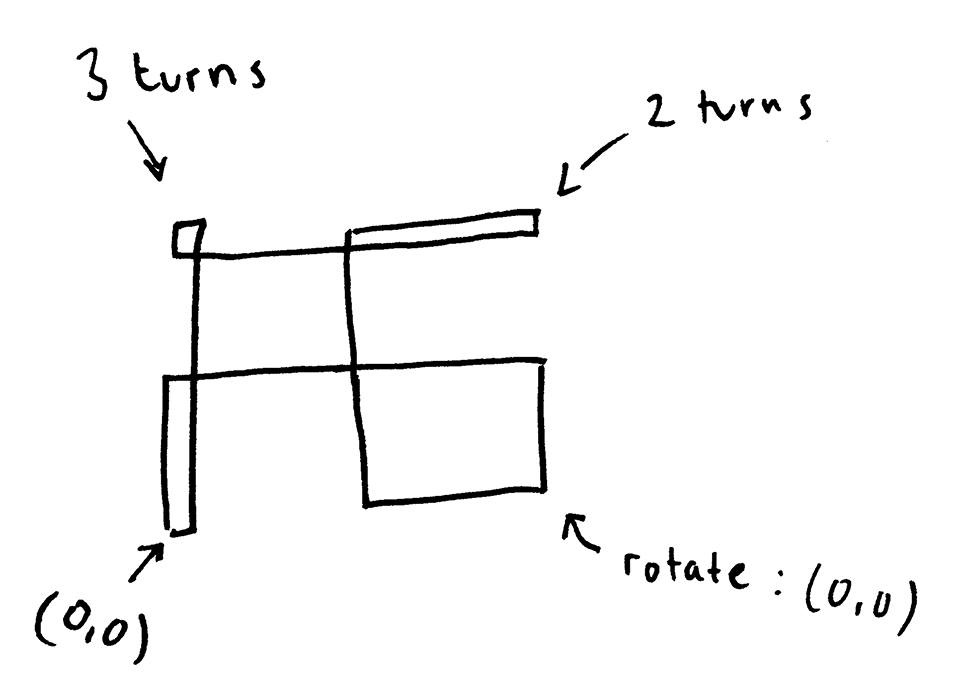
\includegraphics[width=0.8\textwidth]{strategy.png}
	\label{fig:strategy}
\end{figure}

To verify that our strategy was indeed the fastest, we configure the \textit{initialize()} function to call \textit{set\_rules1()}, which configures the model with our strategy.
First, we run the verifier on the following property:

\begin{equation}
	\label{eq:eq}
	E<>(V.in\_initial\_pos() ~ \&\& ~ all\_visited() ~ \&\& ~ total ==  72)
\end{equation}

\textbf{Property \ref{eq:eq} is satisfied} in our configuration.
This tells us that our winning strategy takes 72 units of time (as expected).
To explore whether or not there exists a better strategy, we remove the function call to \textit{set\_rules1()} and allow the model to build any configuration.
Since we have to explore every possible configuration, it does not matter whether the model attempts a depth-first or breadth-first search, and attempting to verify property \ref{eq:leq} will indicate that:

\textbf{Property \ref{eq:leq} is not satisfied} in any configuration.


\begin{equation}
	\label{eq:leq}
	E<>(V.in\_initial\_pos() ~ \&\& ~ all\_visited() ~ \&\& ~ total <=  72)
\end{equation}

Since property \ref{eq:leq} cannot be satisfied in any legal configuration, we can ascertain that no configuration takes less time than $72$ units.
This means that our strategy is indeed the fastest, at $72$ units of time per circuit.

%----------------------------------------------------------------------------------------

\end{document}

